\documentclass[11pt,a4paper]{article}

% PACKAGES FOR TITLES
\usepackage{titlesec}
\usepackage{color}

% PACKAGES FOR LANGUAGE AND FONT
\usepackage[utf8]{inputenc}
\usepackage[english]{babel}
\usepackage[T1]{fontenc} % Font encoding

% PACKAGES FOR IMAGES
\usepackage{graphicx}
\graphicspath{{img/}}
\usepackage{eso-pic} % For the background picture on the title page
\usepackage{subfig} % Numbered and caption subfigures using \subfloat
\usepackage{caption} % Coloured captions
\usepackage{transparent}

% STANDARD MATH PACKAGES
\usepackage{amsmath}
\usepackage{amsthm}
\usepackage{bm}
\usepackage[overload]{empheq}  % For braced-style systems of equations

% PACKAGES FOR TABLES
\usepackage{tabularx}
\usepackage{longtable} % tables that can span several pages
\usepackage{colortbl}

% PACKAGES FOR ALGORITHMS (PSEUDO-CODE)
\usepackage{algorithm}
\usepackage{algorithmic}

% PACKAGES FOR REFERENCES & BIBLIOGRAPHY
\usepackage[colorlinks=true,linkcolor=black,anchorcolor=black,citecolor=black,filecolor=black,menucolor=black,runcolor=black,urlcolor=black]{hyperref} % Adds clickable links at references
\usepackage{cleveref}
\usepackage[square, numbers, sort&compress]{natbib} % Square brackets, citing references with numbers, citations sorted by appearance in the text and compressed
\bibliographystyle{plain} % You may use a different style adapted to your field

% PACKAGES FOR THE APPENDIX
\usepackage{appendix}

% PACKAGES FOR ITEMIZE & ENUMERATES
\usepackage{enumitem}

% OTHER PACKAGES
\usepackage{amsthm,thmtools,xcolor} % Coloured "Theorem"
\usepackage{comment} % Comment part of code
\usepackage{fancyhdr} % Fancy headers and footers
\usepackage{lipsum} % Insert dummy text
\usepackage[skins]{tcolorbox} % Create coloured boxes (e.g. the one for the key-words)
\usepackage{listings}
\usepackage{xcolor}
\usepackage{multicol}

\renewcommand{\footnotesize}{\scriptsize}

\definecolor{codegreen}{rgb}{0,0.6,0}
\definecolor{codegray}{rgb}{0.5,0.5,0.5}
\definecolor{codepurple}{rgb}{0.58,0,0.82}
\definecolor{backcolour}{rgb}{0.95,0.95,0.92}

\lstdefinestyle{mystyle}{
    backgroundcolor=\color{backcolour},
    commentstyle=\color{codegreen},
    keywordstyle=\color{magenta},
    numberstyle=\tiny\color{codegray},
    stringstyle=\color{codepurple},
    basicstyle=\ttfamily\footnotesize,
    breakatwhitespace=false,
    breaklines=true,
    captionpos=b,
    keepspaces=true,
    numbers=none,
    numbersep=5pt,
    showspaces=false,
    showstringspaces=false,
    showtabs=false,
    tabsize=2,
    literate={~} {$\sim$}{1}
}

\lstset{
    style=mystyle
}

\newcommand{\bea}{\begin{eqnarray}} % Shortcut for equation arrays
\newcommand{\eea}{\end{eqnarray}}
\newcommand{\e}[1]{\times 10^{#1}}  % Powers of 10 notation
\newcommand{\mathbbm}[1]{\text{\usefont{U}{bbm}{m}{n}#1}} % From mathbbm.sty
\newcommand{\pdev}[2]{\frac{\partial#1}{\partial#2}}

% Configuration package
\usepackage[bottom=2.0cm,top=2.0cm,left=2.0cm,right=2.0cm]{geometry}
\raggedbottom 

% Create color bluePoli (-> manuale grafica coordinata:  https://www.polimi.it/fileadmin/user_upload/il_Politecnico/grafica-coordinata/2015_05_11_46xy_manuale_grafica_coordinata.pdf)
\definecolor{bluePoli}{cmyk}{0.4,0.1,0,0.4}

% Custom theorem environments
\declaretheoremstyle[
  headfont=\color{bluePoli}\normalfont\bfseries,
  bodyfont=\color{black}\normalfont\itshape,
]{colored}

\captionsetup[figure]{labelfont={color=bluePoli}} % Set colour of the captions
\captionsetup[table]{labelfont={color=bluePoli}} % Set colour of the captions
\captionsetup[algorithm]{labelfont={color=bluePoli}} % Set colour of the captions

\theoremstyle{colored}
\newtheorem{theorem}{Theorem}[section]
\newtheorem{proposition}{Proposition}[section]

% Enhances the features of the standard "table" and "tabular" environments.
\newcommand\T{\rule{0pt}{2.6ex}}
\newcommand\B{\rule[-1.2ex]{0pt}{0pt}}

% Algorithm description
\newcounter{algsubstate}
\renewcommand{\thealgsubstate}{\alph{algsubstate}}
\newenvironment{algsubstates}{
    \setcounter{algsubstate}{0}%
    \renewcommand{\STATE}{%
    \stepcounter{algsubstate}%
    \Statex {\small\thealgsubstate:}\space}
    }{}
    
% Custom theorem environment
\newcolumntype{L}[1]{>{\raggedright\let\newline\\\arraybackslash\hspace{0pt}}m{#1}}
\newcolumntype{C}[1]{>{\centering\let\newline\\\arraybackslash\hspace{0pt}}m{#1}}
\newcolumntype{R}[1]{>{\raggedleft\let\newline\\\arraybackslash\hspace{0pt}}m{#1}}

% Custom itemize environment
\setlist[itemize,1]{label=$\bullet$}
\setlist[itemize,2]{label=$\circ$}
\setlist[itemize,3]{label=$-$}
\setlist{nosep}

% Create command for background pic
\newcommand\BackgroundPic{% Adding background picture
	\put(237,365){
	    \parbox[b][\paperheight]{\paperwidth}{%
	    \vfill
		\centering
		%\transparent{0.4}
		
\includegraphics[width=0.44\paperwidth]{raggiera_polimi.eps}%
		\vfill}
		}
}

% Set indentation
\setlength\parindent{0pt}

% Custom title commands
\titleformat{\section}
{\color{bluePoli}\normalfont\Large\bfseries}
{\color{bluePoli}\thesection.}{1em}{}
\titlespacing*{\section}
{0pt}{3.3ex}{3.3ex}

\titleformat{\subsection}
{\color{bluePoli}\normalfont\large\bfseries}
{\color{bluePoli}\thesubsection.}{1em}{}
\titlespacing*{\subsection}
{0pt}{3.3ex}{3.3ex}

% Custom headers and footers
\pagestyle{fancy}
\fancyhf{}
      
\fancyfoot{}
\fancyfoot[C]{\thepage} % page
\renewcommand{\headrulewidth}{0mm} % headrule width
\renewcommand{\footrulewidth}{0mm} % footrule width

\makeatletter
\patchcmd{\headrule}{\hrule}{\color{black}\hrule}{}{} % headrule
\patchcmd{\footrule}{\hrule}{\color{black}\hrule}{}{} % footrule
\makeatother

\renewcommand{\title}{DWA vs custom trajectory tracking controller: a comparison in ROS}
\newcommand{\AUTHORa}{Giuseppe Chiari}
\newcommand{\IDa}{10576799}
\newcommand{\AUTHORb}{Leonardo Gargani}
\newcommand{\IDb}{10569221}
\newcommand{\AUTHORc}{Serena Salvi}
\newcommand{\IDc}{10607377}
\newcommand{\course}{Computer Science and Engineering}
\newcommand{\supervisor}{Luca Bascetta}
\newcommand{\YEAR}{2022/2023}

\renewcommand{\abstract}{

The Dynamic Window Approach (DWA) is an online collision avoidance strategy for mobile robots.
It incorporates the dynamics of the robot by reducing the search space to only the velocities reachable within a short time interval.

In this work we first present a comparison between the DWA algorithm from the paper and its implementation in Robot Operating System (ROS).

Then, a further comparison is made between the implementation above and a custom trajectory tracking controller, which is composed of an inner linearisation law (based on the kinematic model) and an outer tracking law (based on a proportional integral controller with velocity feed-forward).

}



\begin{document}

\AddToShipoutPicture*{\BackgroundPic}

\hspace{-0.6cm}
\includegraphics[width=0.6\textwidth]{logo_polimi_ing_indinf.eps}

\vspace{-1mm}
\Large{\textbf{\color{bluePoli}{\title}}}\\

\vspace{-0.2cm}
\fontsize{0.3cm}{0.5cm}\selectfont \bfseries \textsc{\color{bluePoli} Project for the Control of Mobile Robots course \\ \course}\\

\vspace{-0.2cm}
\large{\textbf{\AUTHORa, \IDa}}\\
\large{\textbf{\AUTHORb, \IDb}}\\
\large{\textbf{\AUTHORc, \IDc}}

\small \normalfont

\vspace{11pt}

\centerline{\rule{1.0\textwidth}{0.4pt}}

\begin{center}
\begin{minipage}[t]{.24\textwidth}
\begin{minipage}{.90\textwidth}
\noindent
\scriptsize{\textbf{Supervisor:}} \\
\supervisor \\
\\
\textbf{Academic year:} \\
\YEAR \\
\\
\end{minipage}
\end{minipage}
\begin{minipage}{.74\textwidth}
\noindent \textbf{\color{bluePoli} Abstract:} {\abstract}
\end{minipage}
\end{center}

\vspace{12pt}

\newpage

\renewcommand*\contentsname{Table of Contents}
\tableofcontents

\newpage




%--------------------------------------------------------------------------------------------------------------
%                                           INTRODUCTION
%--------------------------------------------------------------------------------------------------------------

\section{Introduction}

%------------------------------------------ PROJECT OVERVIEW ------------------------------------------

\subsection{Project overview}

This project aims at comparing the behavior of a robot when controlled in two different ways: first with a
trajectory tracking controller, and then with the Dynamic Window Approach (DWA).\\

The software performs a simulation of a differential drive robot, using its kinematic model, and implements
the two controllers. To test the quality of the results, an eight-shaped trajectory has been chosen as the
reference one to be followed.\\

Everything runs on \textit{ROS Melodic} on \textit{Ubuntu 18.04}.

%------------------------------------------ BACKGROUND ON DIFFERENTIAL DRIVE ------------------------------------------

\subsection{Background on differential drive}

%$$ \dot{x} = \frac{v_r + v_l}{2} \cos{\theta} $$
%$$ \dot{y} = \frac{v_r + v_l}{2} \sin{\theta} $$
%$$ \dot{\theta} = \frac{v_r - v_l}{L} $$

\begin{multicols}{2}
    $$
    \begin{cases}
        \omega_R = {\frac {v + \omega \cdot d/2}{r}} \\
        \omega_L = {\frac {v - \omega \cdot d/2}{r}}
    \end{cases}
    $$
    \break
    \begin{equation}
        b=c
    \end{equation}
\end{multicols}






%--------------------------------------------------------------------------------------------------------------
%                                               DWA OVERVIEW
%--------------------------------------------------------------------------------------------------------------

\section{DWA overview}

This section contains a brief overview of DWA as presented in the original paper\footnote{\href{https://www.ri.cmu.edu/pub_files/pub1/fox_dieter_1997_1/fox_dieter_1997_1.pdf}{D. Fox, W. Burgard, S. Thrun (1997) \textit{The Dynamic Window Approach to Collision Avoidance}}}.
Basically, it is an approach to perform collision avoidance in mobile robots, while dealing with the constraints
imposed by limited velocities and accelerations.\\

Given a certain goal point to be reached by the robot, DWA tries to find the optimal linear and angular velocities
to go there. This is mainly done in two steps: search space reduction and objective function optimization.


%------------------------------------------ SEARCH SPACE REDUCTION ------------------------------------------

\subsection{Search space reduction}

This approach consists in reducing the search space to those velocities which are reachable under the dynamic constraints and are safe with respect to obstacles.

One of the core concepts of DWA is the so-called search space. It can be seen as a two-dimensional space where
each point represents a tuple $(v, \omega)$ of velocities where $v$ is the linear velocity of the robot and
$\omega$ is the angular velocity.\\

An initial reduction of this space is obtained by searching only in circular trajectories of the robot.

In fact, at each time instant the velocities $(v, \omega)$ are considered constant for the next \textit{n}
time intervals making up the simulated trajectory. The search is repeated after each time interval.\\

The search space is further reduced by considering only all the admissible velocities, which correspond to
the velocities allowing the robot to stop before it reaches the closest obstacle.

Finally, given the limited accelerations of the robot, all the velocities that can't be reached within a short
time interval are left out too.\\


%------------------------------------------ OBJECTIVE FUNCTION OPTIMIZATION ------------------------------------------

\subsection{Objective function optimization}

The remaining velocities are fed into the following objective function to be maximized:
$$ G(v, \omega) = \sigma(\alpha \cdot heading(v, \omega) + \beta \cdot dist(v, \omega) + \gamma \cdot vel(v, \omega)) $$

This function trades off the following aspects:
\begin{itemize}
    \item \textit{heading}, which is a measure of progress towards the goal location;
    \item \textit{dist}, which is the distance to the closest obstacle on the trajectory;
    \item \textit{vel}, which is the forward velocity of the robot.\\
\end{itemize}

Each one of the three quantities above is multiplied to its own weight ($\alpha$, $\beta$, $\gamma$), and the resulting quantity is passed to a smoothing function ($\sigma$).\\

At this point the tuple $(v, \omega)$ leading to the highest score is chosen and the robot picks those velocities.\\




%--------------------------------------------------------------------------------------------------------------
%                                                DWA IN ROS
%--------------------------------------------------------------------------------------------------------------

\section{DWA in ROS}


%------------------------------------------ FROM ROS WIKI ------------------------------------------

\subsection{From ROS wiki}

DWA is already implemented in ROS in the \texttt{dwa\_local\_planner}\footnote{\href{https://wiki.ros.org/dwa\_local\_planner}{https://wiki.ros.org/dwa\_local\_planner}} package.\\

As stated in the ROS Wiki:
\begin{quote}
 ``This package provides a controller that drives a mobile base in the plane. This controller serves to connect the path planner to the robot. Using a map, the planner creates a kinematic trajectory for the robot to get from a start to a goal location. Along the way, the planner creates, at least locally around the robot, a value function, represented as a grid map. This value function encodes the costs of traversing through the grid cells. The controller's job is to use this value function to determine dx,dy,dtheta velocities to send to the robot.''
\end{quote}

This package is ought to be used as the planner for \texttt{move\_base}\footnote{\href{https://wiki.ros.org/move\_base}{https://wiki.ros.org/move\_base}} (package providing an implementation of an action that, given a goal in the world,
will attempt to reach it with a mobile base) within the navigation stack.\\

In the Wiki the following cost function to score each trajectory is presented:

\begin{tcolorbox}[enhanced,width=6in,center,size=fbox]

cost \textbf{=} path\_distance\_bias \textbf{*} (distance to path from the endpoint of the trajectory)\\
    \hspace*{4em}\textbf{+} goal\_distance\_bias \textbf{*} (distance to local goal from the endpoint of the trajectory)\\
    \hspace*{4em}\textbf{+} occdist\_scale \textbf{*} (maximum obstacle cost along the trajectory in obstacle cost (0-254))

\end{tcolorbox}

However, reading through the source code of the DWA ROS library, it is said that the above function is
\textit{``used for visualization only, total\_costs are not really total costs''} \footnote{\href{https://docs.ros.org/en/melodic/api/dwa\_local\_planner/html/dwa\_\_planner\_8cpp\_source.html}{https://docs.ros.org/en/melodic/api/dwa\_local\_planner/html/dwa\_\_planner\_8cpp\_source.html}}.
This is because ROS uses a slightly different cost function that will be described in the next paragraph.


%------------------------------------------ ROS LIBRARY SOURCE CODE ------------------------------------------

\subsection{ROS libray source code}

In order to use DWA in our experiment, we call the \texttt{DWAPlannerROS::computeVelocityCommands()} function which leads to the following cascading function calls:\\
\begin{enumerate}

    \item \texttt{DWAPlannerROS::computeVelocityCommands()}\footnote
    {\href{https://docs.ros.org/en/melodic/api/dwa\_local\_planner/html/dwa\_\_planner\_\_ros\_8cpp\_source.html}
    {https://docs.ros.org/en/melodic/api/dwa\_local\_planner/html/dwa\_\_planner\_\_ros\_8cpp\_source.html}}
    called by \texttt{diffdrive\_traj\_ctrl.cpp} at line 78;

    \item \texttt{DWAPlannerROS::dwaComputeVelocityCommands()}\footnote
    {\href{https://docs.ros.org/en/melodic/api/dwa\_local\_planner/html/dwa\_\_planner\_\_ros\_8cpp\_source.html}
    {https://docs.ros.org/en/melodic/api/dwa\_local\_planner/html/dwa\_\_planner\_\_ros\_8cpp\_source.html}}
    called by function above at line 302;

    \item \texttt{DWAPlanner::findBestPath()}\footnote
    {\href{https://docs.ros.org/en/melodic/api/dwa\_local\_planner/html/dwa\_\_planner\_8cpp\_source.html}
    {https://docs.ros.org/en/melodic/api/dwa\_local\_planner/html/dwa\_\_planner\_8cpp\_source.html}}
    called by function above at line 209;

    \item \texttt{SimpleScoredSamplingPlanner::findBestTrajectory()}\footnote
    {\href{https://docs.ros.org/en/melodic/api/base\_local\_planner/html/simple\_\_scored\_\_sampling\_\_planner\_8cpp\_source.html}
    {https://docs.ros.org/en/melodic/api/base\_local\_planner/html/simple\_\_scored\_\_sampling\_\_planner\_8cpp\_source.html}}
    called by function above at line 317;

    \item \texttt{SimpleScoredSamplingPlanner::scoreTrajectory()}\footnote
    {\href{https://docs.ros.org/en/melodic/api/base\_local\_planner/html/simple\_\_scored\_\_sampling\_\_planner\_8cpp\_source.html}
    {https://docs.ros.org/en/melodic/api/base\_local\_planner/html/simple\_\_scored\_\_sampling\_\_planner\_8cpp\_source.html}}
    called by function above at line 105.\\

\end{enumerate}

At this point, inside \texttt{scoreTrajectory()} the different cost elements are evaluated to score the trajectory.

Each cost element is an instance of the abstract \texttt{base\_local\_planner::TrajectoryCostFunction} class.\\

These elements are contained in a \texttt{std::vector<TrajectoryCostFunction*>} vector and, in the case of DWA, they are
7 in total:

\begin{itemize}
    \item \texttt{base\_local\_planner::OscillationCostFunction oscillation\_costs\_}, which penalizes trajectories where the robot oscillates;
    \item \texttt{base\_local\_planner::ObstacleCostFunction obstacle\_costs\_}, which penalizes trajectories where the robot occupies illegal positions with its footprint;
    \item \texttt{base\_local\_planner::MapGridCostFunction goal\_front\_costs\_}, which prefers  trajectories that make the nose go towards (local) nose goal;
    \item \texttt{base\_local\_planner::MapGridCostFunction alignment\_costs\_}, which prefers trajectories that keep the robot nose on nose path;
    \item \texttt{base\_local\_planner::MapGridCostFunction path\_costs\_}, which prefers trajectories on global path;
    \item \texttt{base\_local\_planner::MapGridCostFunction goal\_costs\_}, which prefers trajectories that go towards (local) goal;
    \item \texttt{base\_local\_planner::TwirlingCostFunction twirling\_costs\_}, which prefers trajectories that don't spin.\\
\end{itemize}

The considered trajectories by DWA are those taken from a equi-distant discretization of the velocities that the robot can assume. For this purpose ROS has a \texttt{base\_local\_planner::SimpleTrajectoryGenerator}\footnote{\href{https://docs.ros.org/en/melodic/api/base\_local\_planner/html/classbase\_\_local\_\_planner\_1\_1SimpleTrajectoryGenerator.html}{https://docs.ros.org/en/melodic/api/base\_local\_planner/html/classbase\_\_local\_\_planner\_1\_1SimpleTrajectoryGenerator.html}} class.


WEIGHTED SUM... (descrivi la funzione di costo implementata nella libreria)



%--------------------------------------------------------------------------------------------------------------
%                                        TRAJECTORY TRACKING CONTROLLER
%--------------------------------------------------------------------------------------------------------------

\section{Trajectory tracking controller}

...


%--------------------------------------------------------------------------------------------------------------
%                                           SETUP OF THE EXPERIMENT
%--------------------------------------------------------------------------------------------------------------

\section{Setup of the experiment}


%------------------------------------------ THE ROBOT ------------------------------------------

\subsection{The robot}

In our experiment we chose to simulate a small differential drive robot.\\

In particular, it is characterized by two main dimensions (specified as YAML parameters in the code):
\begin{itemize}
    \item \texttt{d} = 15 cm, which is the distance between the two motorized wheels;
    \item \texttt{r} = 3 cm, which is the radius of the two motorized wheels.\\
\end{itemize}

The precise footprint is a pentagon, just for convenience, so that when looking at it we are able to determine the orientation of the robot.
However, this is not a decisive detail since it has o influence on the robot's behavior.


%------------------------------------------ THE MAP ------------------------------------------

\subsection{The map}

Regarding the map, it is important to highlight the different setting we have with respect to the usual DWA use.

There are two main differences:
\begin{itemize}
    \item in our setting there are no obstacles, neither fixed nor moving;
    \item the robot does not have any sensor.\\
\end{itemize}

As a consequence, we don't need both the local map and the global map, but only the local one.

Moreover, this map needs to be empty so it is generated starting from a totally white image.


%------------------------------------------ THE TRAJECTORY ------------------------------------------

\subsection{The trajectory}

The robot must follow a precise trajectory, which is used to perform all benchmarks.

In our case we chose an eight-shaped trajectory with a dimension of 2 x 1 meters.\\

In order to make DWA compute the velocities of the robot, we must feed it a goal.

This means that the complete trajectory has to be "discretized" in multiple points.
Each one of these points is passed to DWA as the current goal, and once it is reached the next point is set as the new goal. You will find a detailed explanation in the following sections.




%--------------------------------------------------------------------------------------------------------------
%                                           IMPLEMENTATION
%--------------------------------------------------------------------------------------------------------------

\section{Implementation}


%------------------------------------------ ARCHITECTURE OVERVIEW ------------------------------------------

\subsection{Architecture overview}

Our implementation is composed of three packages: one simulator (\texttt{diffdrive\_kin\_sim}) and two controllers (\texttt{diffdrive\_kin\_ctrl} and \texttt{diffdrive\_dwa\_ctrl}).

The two controllers are interchangeable and are meant to always be used together with the simulator, one at a time.

\subsection{Service}

\subsubsection{\texttt{generate\_desired\_path\_service}}

The 8-shaped trajectory that the robot must follow is generated inside \texttt{eight\_traj\_gen.cpp} executed in the launch file.

As a result, the two vectors contained in the \texttt{GenerateDesiredPathService.srv} message are populated with the coordinates of all the points of the trajectory.

As soon as the service is called, during the initialization (in the \texttt{Prepare()} function) of both controllers, the complete trajectory is made available also to the controllers.


%------------------------------------------ NODES ------------------------------------------

\subsection{Nodes}

\subsubsection{\texttt{diffdrive\_kin\_sim\_node}}

This node is subscribed to the \texttt{/robot\_input} topic and reads the wheels velocities.

Given those it simulates the movement of the robot and publishes the new position in both \texttt{/robot\_state} and \texttt{/odom} topics. We have decided to keep these two topics separate in order to accommodate both controllers.\\

The actual simulator is an object of the \texttt{diffdrive\_kin\_ode} class, which is initialized as follow:
\begin{lstlisting}
simulator = new diffdrive_kin_ode(dt);
\end{lstlisting}

and contains the integration logic to update the robot pose.

\subsubsection{\texttt{diffdrive\_kin\_trajctrl\_node}}

This node is dedicated to compute the angular velocities of the two wheels given the current position of the robot and its next point in the trajectory.\\

During the initialization phase it queries the \texttt{generate\_desired\_path\_service} service and stores the complete trajectory.

Then, every time a message is published on the \texttt{/robot\_state} topic this node updates its internal values of the robot pose.\\

The \texttt{PeriodicTask()} that gets executed uses a PID controller and a linearization law (implemented in the \texttt{diffdrive\_kin\_fblin} class) to compute both the linear and the angular velocities of the robot.

As a last step, since the simulated robot is a differential drive one, the angular velocities of the two wheels are computed starting from the $(v, \omega)$ above, and the new results are published on the \texttt{/robot\_input} and \texttt{/controller\_state} topics.

\subsubsection{\texttt{diffdrive\_dwa\_trajctrl\_node}}

This node is used to interface the DWA library in ROS with the simulator.

This is due to the fact that natively DWA is used inside ROS Navigation Stack, thus it expects an odometry source and a costmap.\\

In this specific implementation only a global costmap and a planner (DWA) are used.

As the controller explained above, during the initialiation phase the service is queried. Once the trajectory is received, one point every \texttt{skipped\_goals} is set as the new plan for DWA.

Once the plan is set, the DWA controller tries to reach the new goal position by computing the necessary pair of $(v, \omega)$ velocities. As soon as the goal is reached with a certain tolerance, the next point in the trajectory is set as the new goal.\\

Lastly, the $(\omega_r,\omega_l)$ velocities are computed and published on the \texttt{/robot\_input} and \texttt{/controller\_state} topics.

The implementation of DWA and all the functions that have been used is provided by the following two files in the ROS library:
\begin{itemize}
    \item \href{https://docs.ros.org/en/melodic/api/dwa\_local\_planner/html/dwa\_\_planner\_8cpp\_source.html}{\texttt{dwa\_planner.cpp}}
    \item \href{https://docs.ros.org/en/melodic/api/dwa\_local\_planner/html/dwa\_\_planner\_\_ros\_8cpp\_source.html}{\texttt{dwa\_planner\_ros.cpp}}
\end{itemize}

\begin{figure}[H]
    \centering
    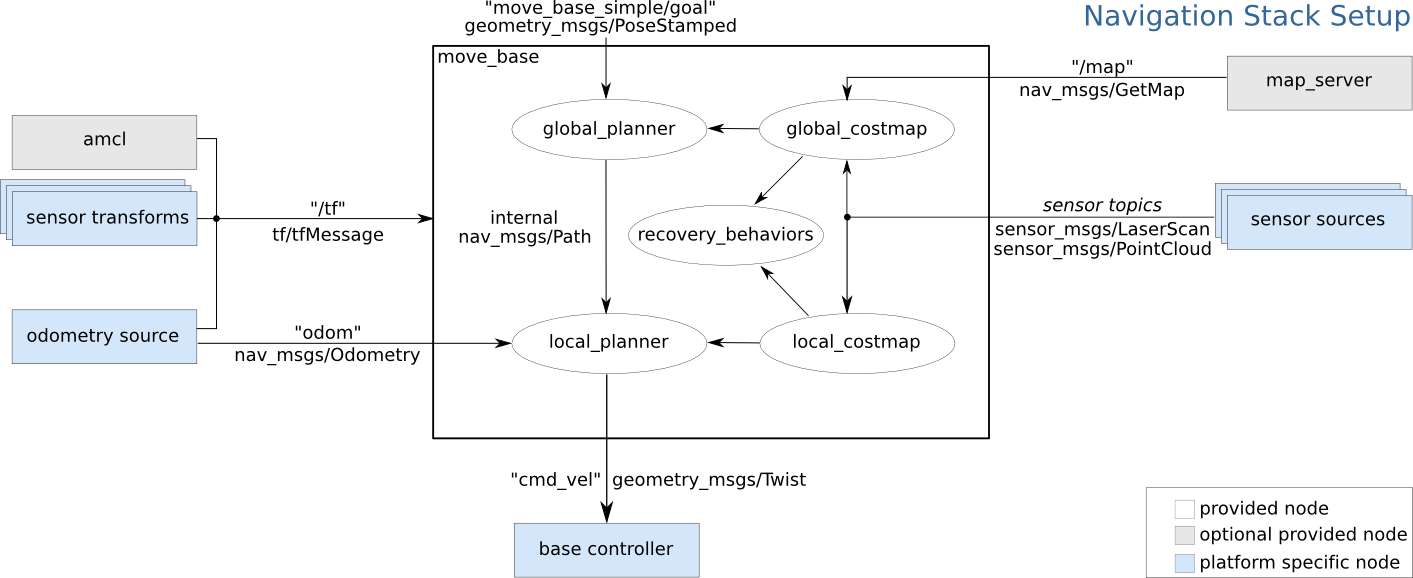
\includegraphics[scale=0.4]{other/navigation_stack.png}
    \caption{ROS Navigation Stack.}
\end{figure}

\subsubsection{\texttt{odom\_to\_baselink\_tf\_node}}

This node is needed in order to link the \texttt{odom} and the \texttt{base\_link} coordinate frames through a simple dynamic tf.


%------------------------------------------ FRAMES ------------------------------------------

\subsection{Frames}

Here is a list with a brief description of all the frames:
\begin{itemize}
    \item \texttt{map}, which is the coordinate system where the empty map (provided by the map server) is;
    \item \texttt{odom}, which represent the global reference system, that in this particular case its origin matches the one of the \texttt{map} frame;
    \item \texttt{base\_link}, which represrents reference system moving around together with the robot.
\end{itemize}

\begin{figure}[H]
    \centering
    \subfloat[\texttt{rqt\_tf\_tree} of the custom controller.]{
        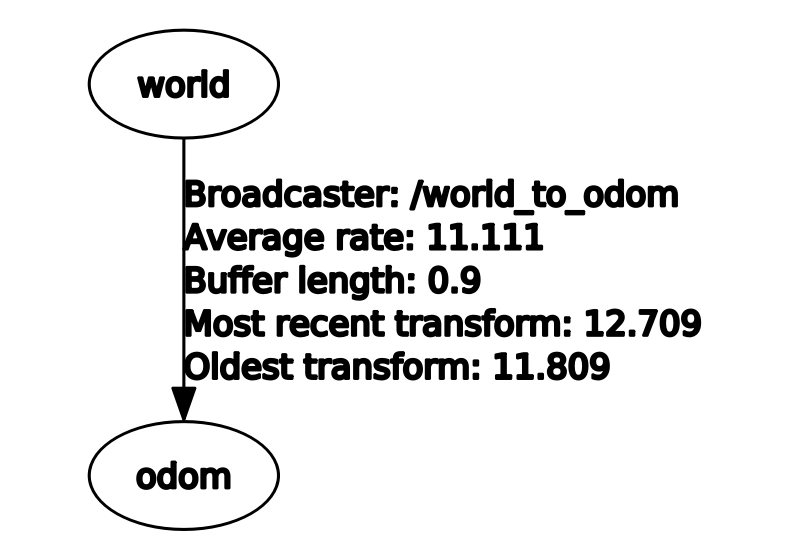
\includegraphics[scale=0.28]{ros_tools/rqttftree_custom.png}
    }
    \subfloat[\texttt{rqt\_tf\_tree} of DWA standalone.]{
        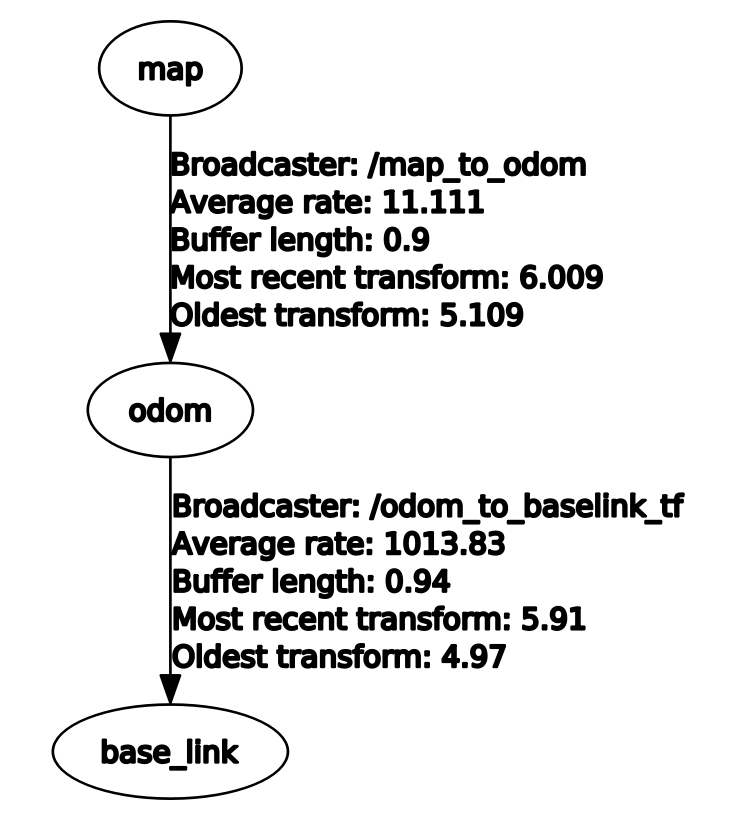
\includegraphics[scale=0.26]{ros_tools/rqttftree_dwa.png}
    }
    \caption[]{Frames in the two approaches.}
\end{figure}


%------------------------------------------ TOPICS ------------------------------------------

\subsection{Topics}

Here is a list with a brief description of the topics that our nodes are subscribed to and published into:\\

\begin{itemize}

    \item \texttt{/clock}, used to synchronize all the nodes in the simulation;

    \item \texttt{/odom}, used to pass the odometry information of the robot to DWA;
        \begin{itemize}
            \item publishers:
                \begin{itemize}
                    \item \texttt{diffdrive\_kin\_sim}
                \end{itemize}
            \item subscribers:
                \begin{itemize}
                    \item \texttt{odom\_to\_baselink\_tf}
                \end{itemize}
        \end{itemize}

    \item \texttt{/robot\_state}, used to pass the odometry information of the robot to the custom controller.
        \begin{itemize}
            \item publishers:
                \begin{itemize}
                    \item \texttt{diffdrive\_kin\_sim}
                \end{itemize}
            \item subscribers:
                \begin{itemize}
                    \item \texttt{diffdrive\_kin\_trajctrl}
                \end{itemize}
        \end{itemize}

    \item \texttt{/controller\_state}, used to publish details about the controller for visualization purposes;
        \begin{itemize}
            \item publishers:
                \begin{itemize}
                    \item \texttt{diffdrive\_kin\_trajctrl}
                    \item \texttt{diffdrive\_dwa\_trajctrl}
                \end{itemize}
            \item subscribers:
                \begin{itemize}
                    \item \textit{none}
                \end{itemize}
        \end{itemize}

    \item \texttt{/robot\_input}, used to communicate $(\omega_r,\omega_l)$ computed by the controllers;
        \begin{itemize}
            \item publishers:
                \begin{itemize}
                    \item \texttt{diffdrive\_kin\_trajctrl}
                    \item \texttt{diffdrive\_dwa\_trajctrl}
                \end{itemize}
            \item subscribers:
                \begin{itemize}
                    \item \texttt{diffdrive\_kin\_sim}
                \end{itemize}
        \end{itemize}

\end{itemize}


%------------------------------------------ LAUNCH FILES ------------------------------------------

\subsection{Launch files}

Here is a list with a brief description of all the launch files:\\
\begin{itemize}
    \item \texttt{diffdrive\_kin\_trajctrl.launch}, used to start the following nodes:
        \begin{itemize}
            \item \texttt{diffdrive\_kin\_sim}
            \item \texttt{diffdrive\_kin\_trajctrl}
            \item \texttt{eight\_traj\_gen}
            \item \texttt{world\_to\_odom} (static tf linking \texttt{world} and \texttt{odom} frames)
            \item \texttt{odom\_visualizer} (\textit{RVIZ} node to visualize data)\\
        \end{itemize}

    \item \texttt{diffdrive\_dwa\_trajctrl.launch}, used to start the following nodes:
        \begin{itemize}
            \item \texttt{diffdrive\_kin\_sim}
            \item \texttt{diffdrive\_dwa\_trajctrl}
            \item \texttt{eight\_traj\_gen}
            \item \texttt{odom\_to\_baselink\_tf}
            \item \texttt{map\_node} (\textit{map\_server} node used to provide the map)
            \item \texttt{map\_to\_odom} (static tf linking \texttt{map} and \texttt{odom} frames)
            \item \texttt{odom\_visualizer} (\textit{RVIZ} node to visualize data)
        \end{itemize}
\end{itemize}

\begin{figure}[H]
    \centering
    \subfloat[\texttt{rqt\_graph} of the custom controller.]{
        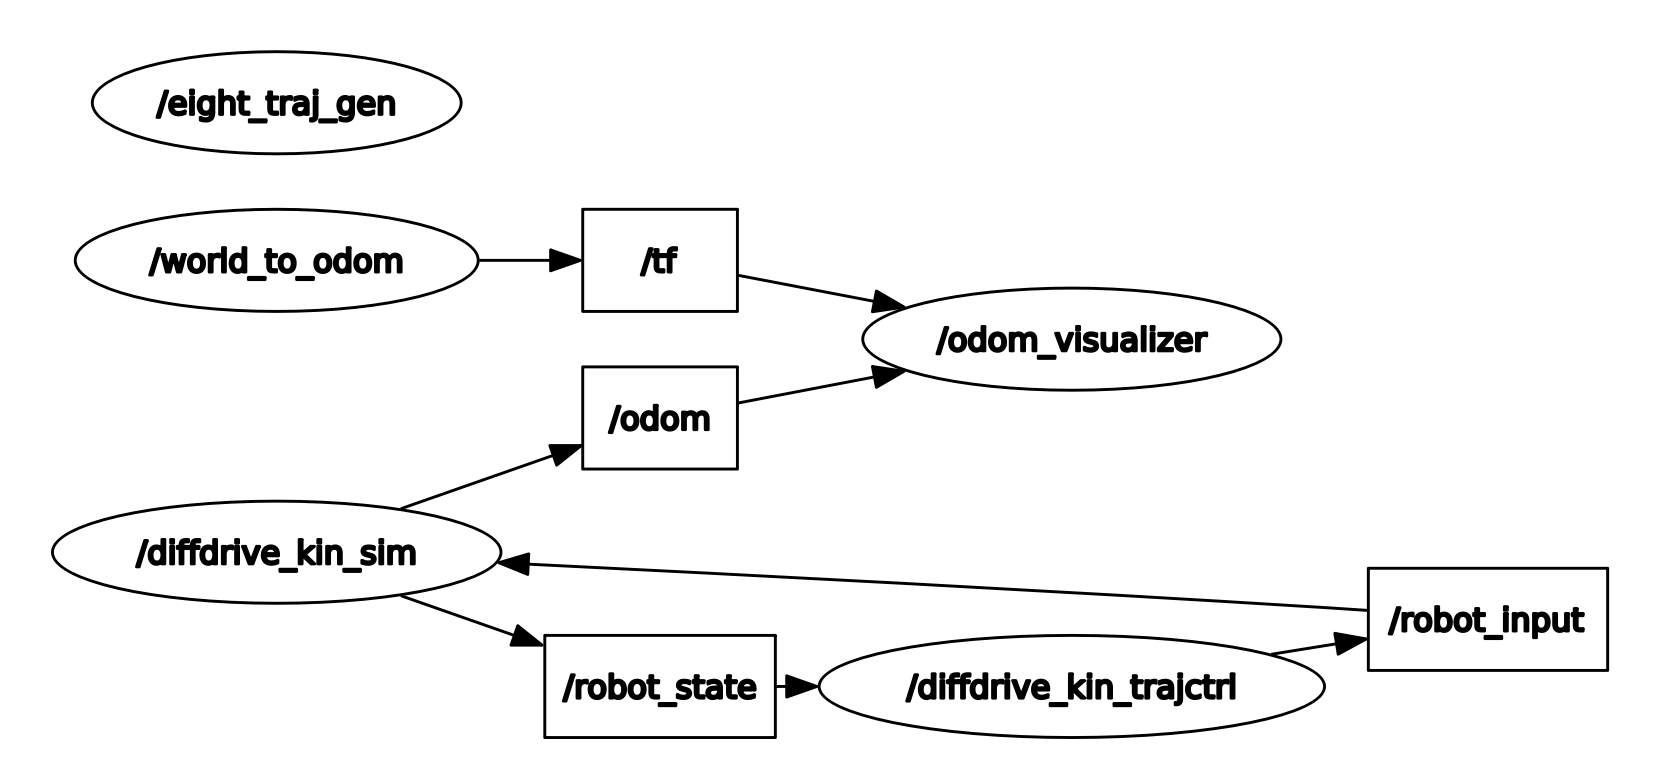
\includegraphics[scale=0.24]{ros_tools/rqtgraph_custom.png}
    }
    \quad
    \subfloat[\texttt{rqt\_graph} of DWA standalone.]{
        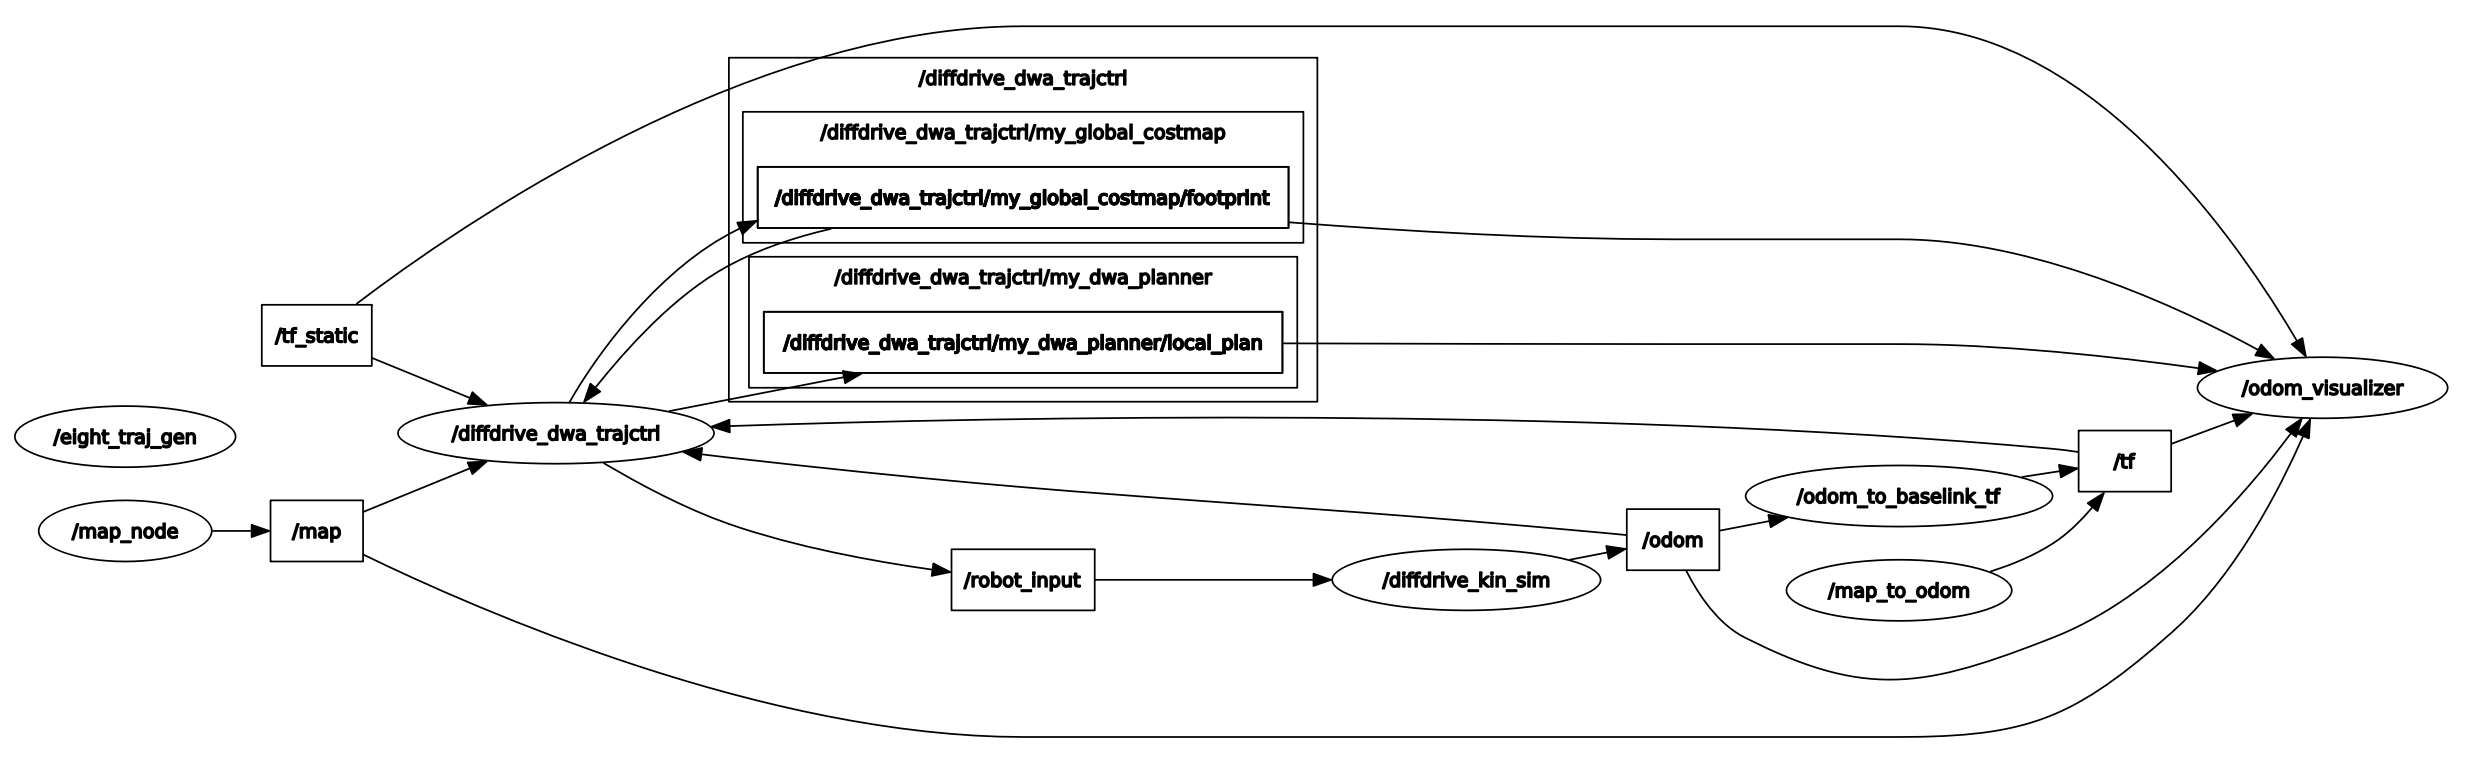
\includegraphics[scale=0.26]{ros_tools/rqtgraph_dwa.png}
    }
    \caption[]{Architecture of the two approaches.}
\end{figure}




%--------------------------------------------------------------------------------------------------------------
%                                               PARAMETERS
%--------------------------------------------------------------------------------------------------------------

\section{Parameters}


%------------------------------------------ LIST OF PARAMETERS ------------------------------------------

\subsection{List of parameters}

Parameters have a crucial role for the correct functioning of the nodes introduced above.\\

In this section the most relevant ones are explained:\\
\begin{itemize}

    \item \texttt{diffdrive\_kin\_sim.yaml}:
        \begin{itemize}
            \item \texttt{d}, distance between the two wheels;
            \item \texttt{r}, radius of the two wheels.\\
        \end{itemize}

    \item \texttt{eight\_traj.yaml}:
        \begin{itemize}
            \item \texttt{a}, amplitude of the eight-shaped trajectory;
            \item \texttt{w}, ratio $\frac{2 \cdot \pi }{T}$ where $T$ is the time duration of each lap;
            \item \texttt{trajectory\_length}, length of the eight-shaped trajectory;
            \item \texttt{increment\_step}, increment step when discretizing the trajectory.\\
        \end{itemize}

    \item \texttt{diffdrive\_kin\_trajctrl.yaml}:
        \begin{itemize}
            \item \texttt{Kp}, proportional gain of the PID controller;
            \item \texttt{Ki}, integral gain of the PID controller;
            \item \texttt{Kd}, derivative gain of the PID controller.\\
        \end{itemize}

    \item \texttt{diffdrive\_dwa\_trajctrl.yaml}:
        \begin{itemize}
            \item \texttt{skipped\_goals}, number of points to skip when feeding the trajectory to DWA.\\
        \end{itemize}

    \item \texttt{dwa\_planner\_params.yaml}:
        \begin{itemize}
            \item \texttt{min\_vel\_y}, minimum linear velocity along the y-axis;
            \item \texttt{max\_vel\_y}, maximum linear velocity along the y-axis;
            \item \texttt{min\_vel\_x}, minimum linear velocity along the x-axis;
            \item \texttt{max\_vel\_x}, minimum linear velocity along the x-axis;
            \item \texttt{acc\_lim\_theta}, maximum angular acceleration;
            \item \texttt{vth\_samples}, number of uniformly-sampled values of $\omega$ that DWA considers when simulating;
            \item \texttt{vx\_samples}, number of uniformly-sampled values of $v$ that DWA considers when simulating;
            \item \texttt{path\_distance\_bias}, weighting for how much the controller should stay close to the given path;
            \item \texttt{goal\_distance\_bias}, weighting for how much the controller should attempt to reach its local goal;
            \item \texttt{xy\_goal\_tolerance}, tolerance (in meters) in the x \& y distance when reaching a goal;
            \item \texttt{yaw\_goal\_tolerance}, tolerance (in radians) in yaw/rotation when reaching a goal.\\
        \end{itemize}

\end{itemize}


%------------------------------------------ TUNING ------------------------------------------

\subsection{Tuning}

\subsubsection{Eight-shaped trajectory}

An eight-shaped trajectory can be be described with the following analytical equations:
$$x = \texttt{a} \cdot \sin (\texttt{w} \cdot t)$$
$$y = \texttt{a} \cdot \sin (\texttt{w} \cdot t)\cdot \cos (\texttt{w} \cdot t)$$\\

In the equations above it is possible to tune two parameters: \texttt{a} and \texttt{w}.
In the presented implementation they are set to \texttt{a} = 1 and \texttt{w} = 1.

\begin{figure}[H]
    \centering
    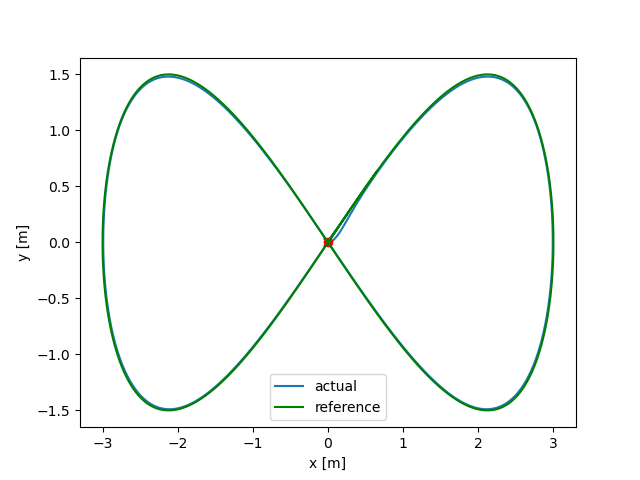
\includegraphics[scale=0.5]{different_params/custom_a3/Trajectory.png}
    \caption{Trajectory when \texttt{a = 3.0}.}
\end{figure}

\subsubsection{Custom controller}

The custom controller is a trajectory tracking one composed of an inner linearisation law and an outer tracking law.
The outer tracking law is based on a PID controller with tunable parameters: $K_p$, $K_i$, $K_d$.\\

The step response when using a PID controller is computed as follows:
$$ {\displaystyle u(t)=K_{\text{p}}e(t)+K_{\text{i}}\int _{0}^{t}e(\tau )\,\mathrm {d} \tau +K_{\text{d}}{\frac {\mathrm {d} e(t)}{\mathrm {d} t}}} $$\\

\begin{figure}[H]
    \centering
    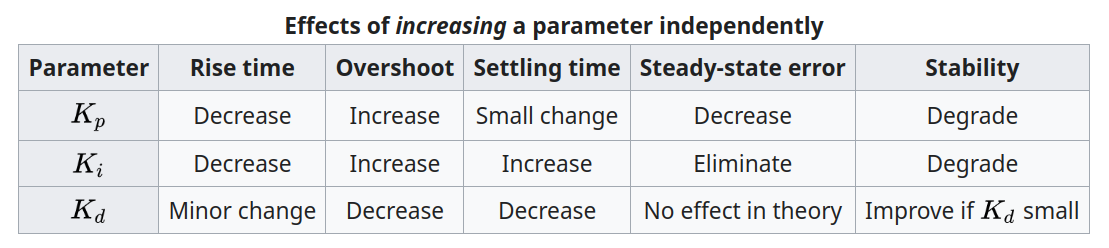
\includegraphics[scale=0.4]{other/PID_parameters_description.png}
    \caption{PID parameters tuning.}
\end{figure}

Various tests have been carried out to achieve the optimal behaviour, in particular to minimize the overshoot and
the settling time while keeping an overall good stability in the PID response.\\

In the presented implementation they are set to $K_p = 0.8$, $K_i = 0.8$, $K_d = 0$.

\begin{figure}[H]
    \centering
    \subfloat[Trajectory.]{
        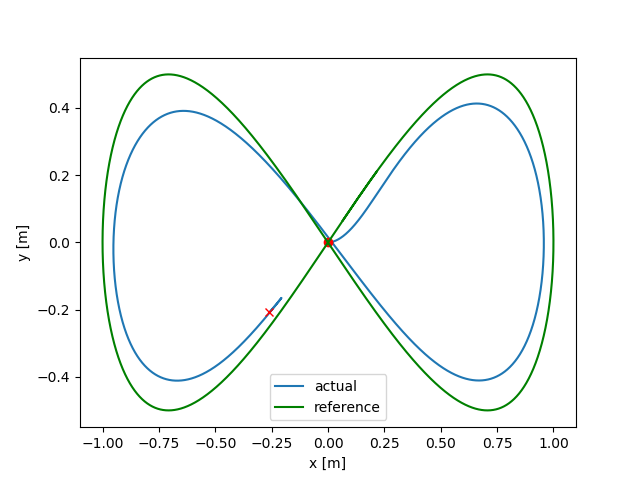
\includegraphics[scale=0.5]{different_params/custom_kp02/Trajectory.png}
    }
    \subfloat[Linear and angular velocities.]{
        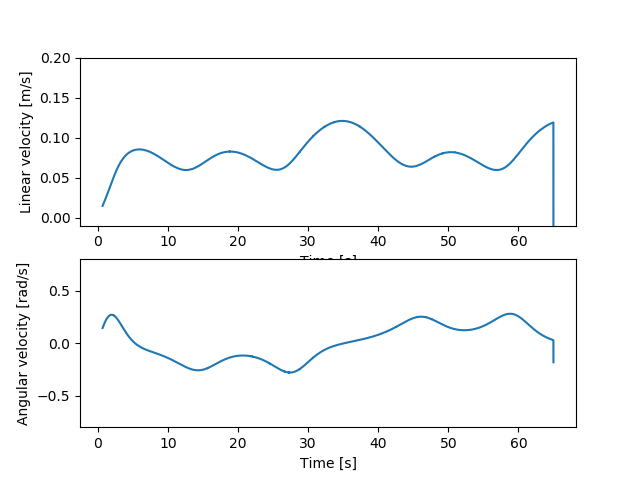
\includegraphics[scale=0.5]{different_params/custom_kp02/Linear_and_Angular_Velocities.png}
    }
    \caption[]{Behavior with $K_p=0.2, K_p=0.8, K_p=0.0$.}
\end{figure}

\begin{figure}[H]
    \centering
    \subfloat[Trajectory.]{
        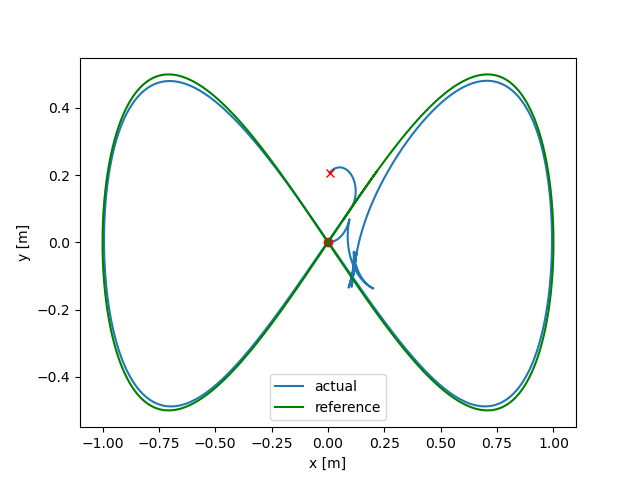
\includegraphics[scale=0.5]{different_params/custom_ki32kd10/Trajectory.png}
    }
    \subfloat[Linear and angular velocities.]{
        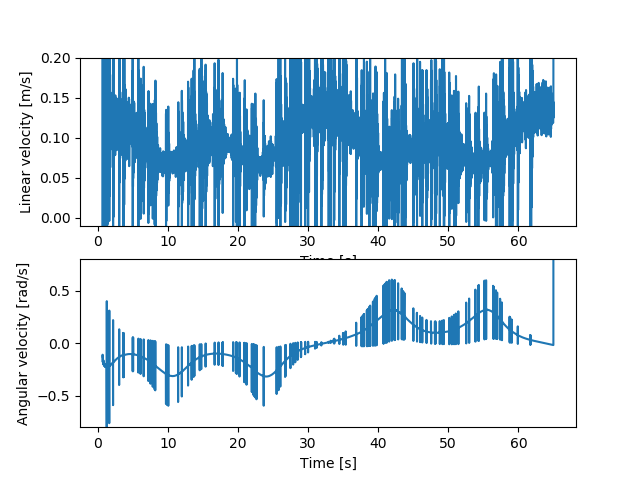
\includegraphics[scale=0.5]{different_params/custom_ki32kd10/Linear_and_Angular_Velocities.png}
    }
    \caption[]{Behavior with $K_p=0.8, K_p=3.2, K_p=1.0$.}
\end{figure}

\subsubsection{DWA}

When the trajectory is generated, the eight shape is discretized over numerous points.

Due to the large number of those, they are very close to each other. This makes the robot misbehave as soon as
a new goal is set in DWA. For this reason it is best to skip some of the points in the trajectory.
This is accomplished through the \texttt{skipped\_goals} parameters, which is set to 15.\\

\begin{figure}[H]
    \centering
    \subfloat[Trajectory.]{
        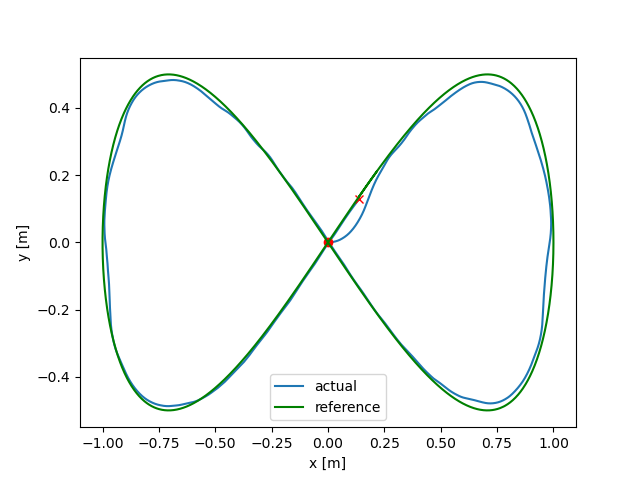
\includegraphics[scale=0.5]{different_params/dwa_skippedgoals0/Trajectory.png}
    }
    \subfloat[Position Error.]{
        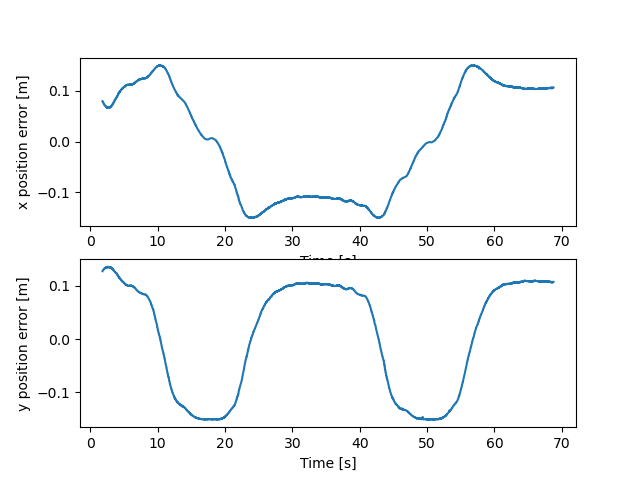
\includegraphics[scale=0.5]{different_params/dwa_skippedgoals0/Position_Error.png}
    }
    \quad
    \subfloat[Linear and angular velocities.]{
        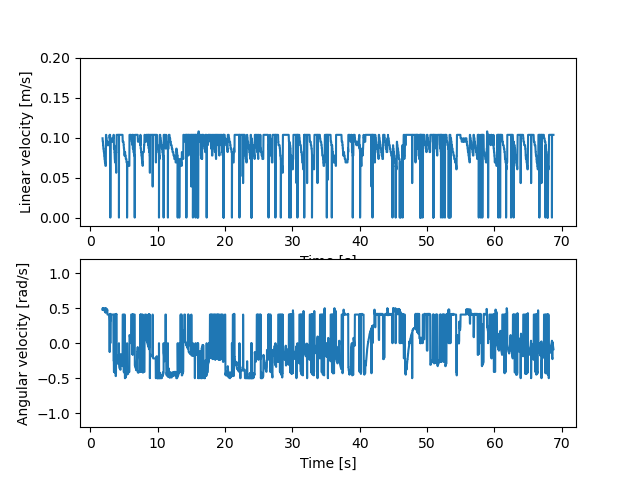
\includegraphics[scale=0.5]{different_params/dwa_skippedgoals0/Linear_and_Angular_Velocities.png}
    }
    \caption[]{Behavior with \texttt{skipped\_goals = 0}.}
\end{figure}

\begin{figure}[H]
    \centering
    \subfloat[Trajectory.]{
        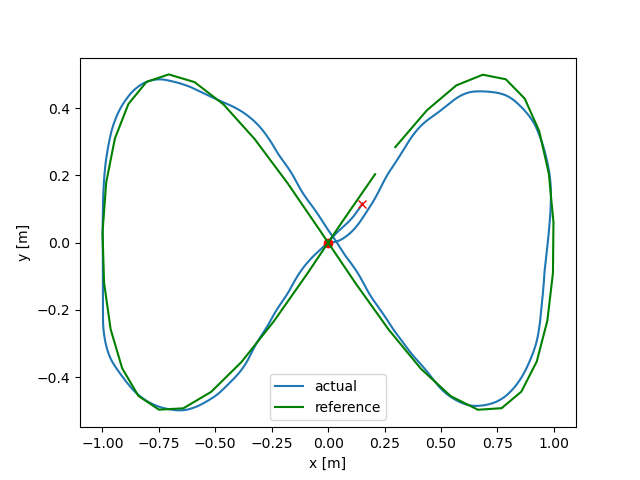
\includegraphics[scale=0.5]{different_params/dwa_skippedgoals150/Trajectory.png}
    }
    \subfloat[Position Error.]{
        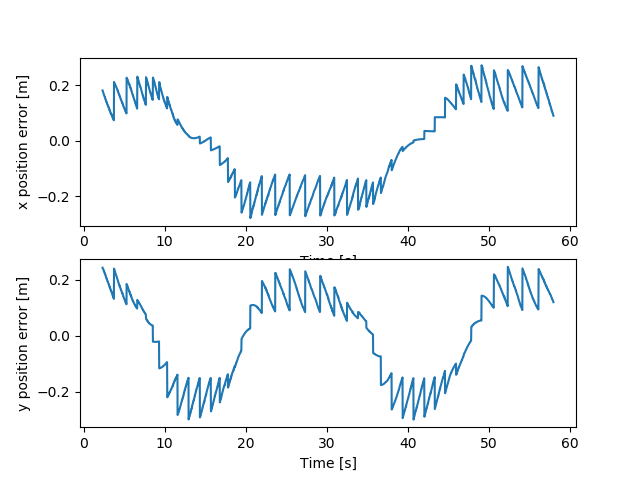
\includegraphics[scale=0.5]{different_params/dwa_skippedgoals150/Position_Error.png}
    }
    \quad
    \subfloat[Linear and angular velocities.]{
        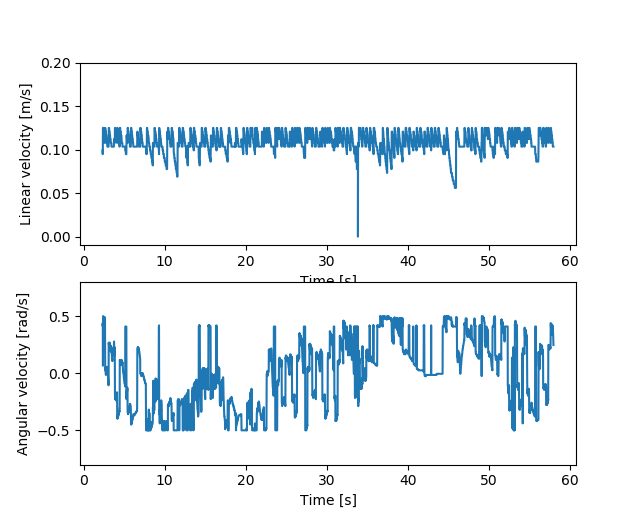
\includegraphics[scale=0.5]{different_params/dwa_skippedgoals150/Linear_and_Angular_Velocities.png}
    }
    \caption[]{Behavior with \texttt{skipped\_goals = 150}.}
\end{figure}

In order to simulate a differential drive robot, the following parameters have been set:

\begin{itemize}
    \item \texttt{min\_vel\_y} = 0 and \texttt{max\_vel\_y} = 0, to forbid lateral movement along the y-axis;
    \item \texttt{min\_vel\_x} = 0, to forbid backward movement along the x-axis.\\
\end{itemize}

Another parameter related to the constraints on the movement of the robot is \texttt{acc\_lim\_theta}.
To achieve the best trade-off betweeen the ability to correctly follow the trajectory and the realistic
constraints on the steering capabilities of the robot, the most suitable value for it is 10.\\

Since DWA discretely sample in the robot's control space, parameters \texttt{vth\_samples} and \texttt{vx\_samples}
play a key role in allowing a finer grained choice of velocities.
To achieve the best trade-off betweeen a wide choice of possible $(v,\omega)$ and computational effort,
the optimal values have been found to be \texttt{vth\_samples = 100} and \texttt{vx\_samples = 30}.\\

Finally, DWA provides a certain tolerance within which the goal is considered to be reached.
In particular this can be done through two parameters \texttt{yaw\_goal\_tolerance} and \texttt{xy\_goal\_tolerance}.
The former has been set to \texttt{6.3} because it is irrelevant the direction of the robot when reaching the goal
(thus $6.3 \simeq 2\pi$ in radians).
The latter has been set to \texttt{0.15} because it is a good deal between the dimension of the robot and
an approximation of the trajectory.




%--------------------------------------------------------------------------------------------------------------
%                                           EXPERIMENTAL RESULTS
%--------------------------------------------------------------------------------------------------------------

\section{Experimental Results}

%--------------------------------------- TUNED TRAJECTORY TRACKING CONTROLLER ---------------------------------------

\subsection{Tuned trajectory tracking controller}

Here are the final results obtained with the optimal parameters in the trajectory tracking controller:

\begin{figure}[H]
    \centering
    \subfloat[Trajectory.]{
        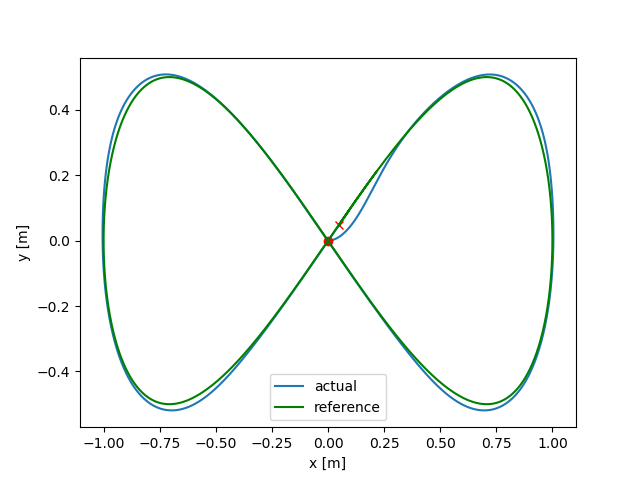
\includegraphics[scale=0.6]{kin_screenshots/Trajectory.png}
    }
    \quad
    \subfloat[Linear and angular velocities.]{
        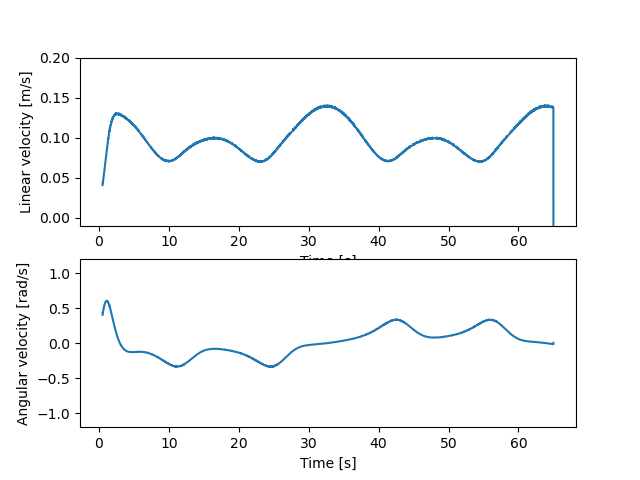
\includegraphics[scale=0.5]{kin_screenshots/Linear_and_Angular_Velocities.png}
    }
    \subfloat[Wheels velocities.]{
        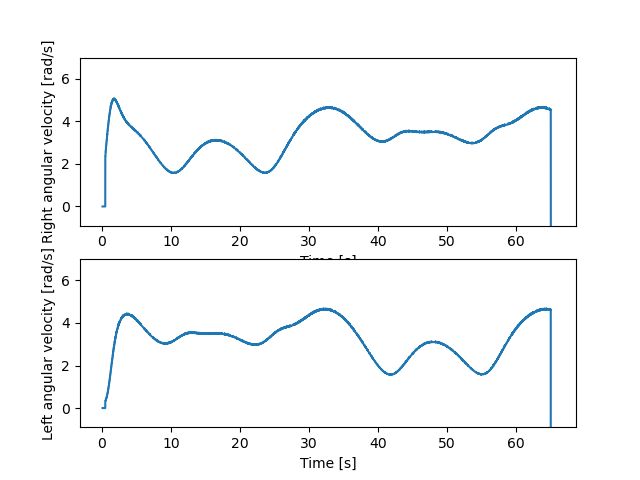
\includegraphics[scale=0.5]{kin_screenshots/Wheels_Velocities.png}
    }
    \quad
    \subfloat[Pose.]{
        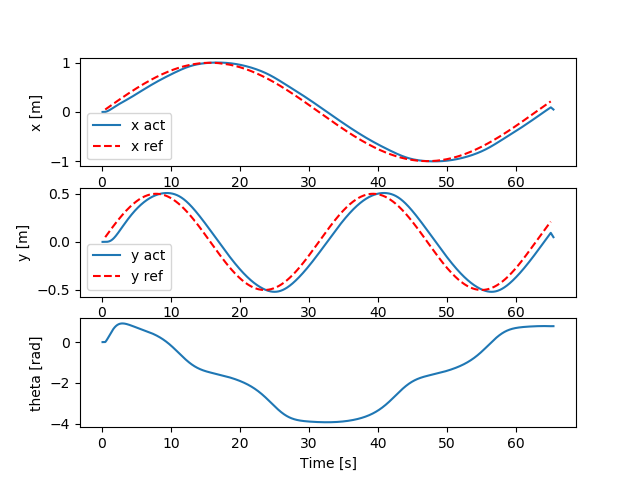
\includegraphics[scale=0.5]{kin_screenshots/Pose.png}
    }
    \subfloat[Position Error.]{
        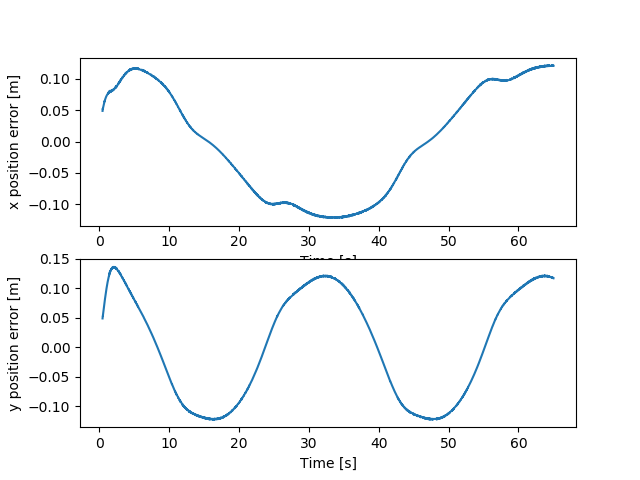
\includegraphics[scale=0.5]{kin_screenshots/Position_Error.png}
    }
    \caption[]{Behavior with the tuned custom controller.}
\end{figure}

%------------------------------------------ TUNED DWA ------------------------------------------

\subsection{Tuned DWA}

Here are the final results obtained with the optimal parameters in DWA:

\begin{figure}[H]
    \centering
    \subfloat[Trajectory.]{
        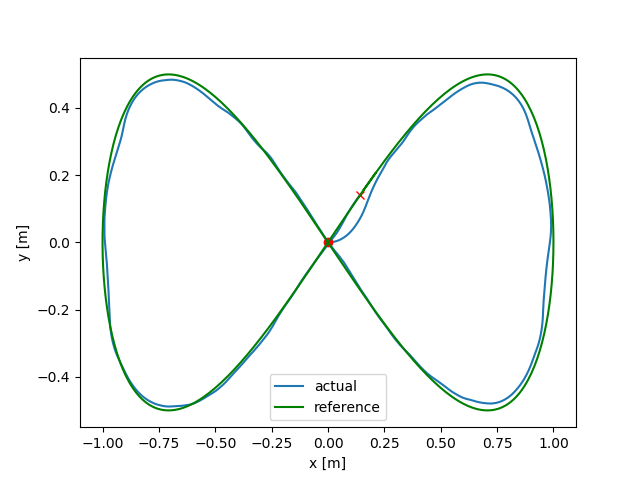
\includegraphics[scale=0.6]{dwa_screenshots/Trajectory.png}
    }
    \quad
    \subfloat[Linear and angular velocities.]{
        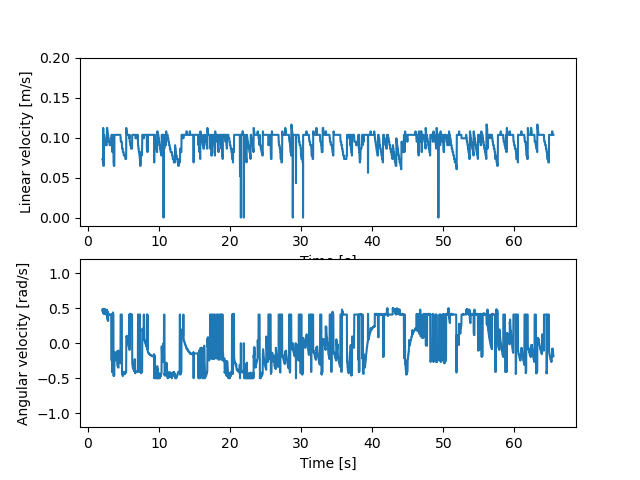
\includegraphics[scale=0.5]{dwa_screenshots/Linear_and_Angular_Velocities.png}
    }
    \subfloat[Wheels velocities.]{
        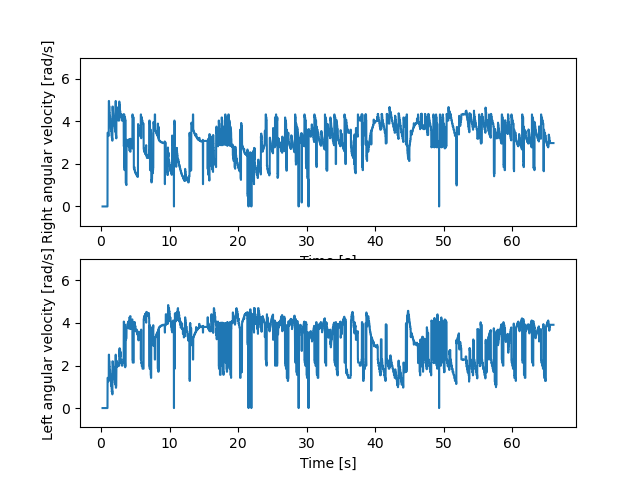
\includegraphics[scale=0.5]{dwa_screenshots/Wheels_Velocities.png}
    }
    \quad
    \subfloat[Pose.]{
        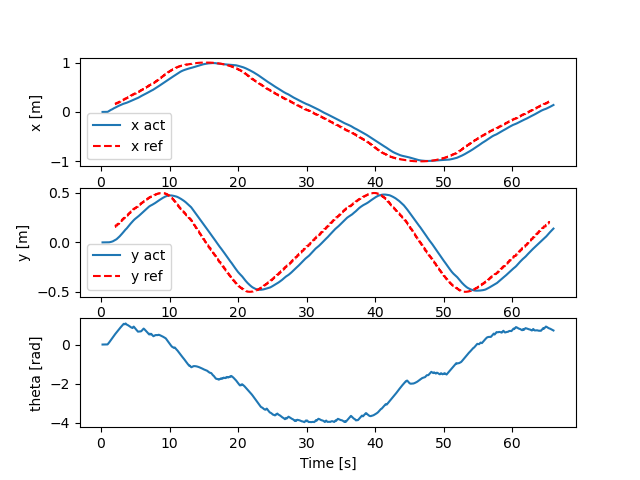
\includegraphics[scale=0.5]{dwa_screenshots/Pose.png}
    }
    \subfloat[Position Error.]{
        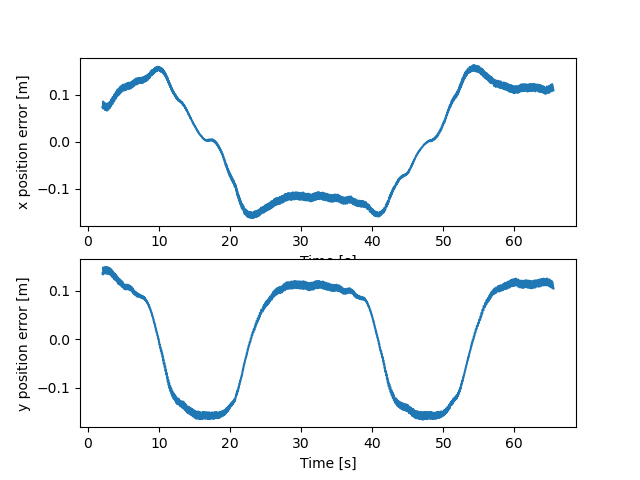
\includegraphics[scale=0.5]{dwa_screenshots/Position_Error.png}
    }
    \caption[]{Behavior with tuned DWA.}
\end{figure}

%------------------------------------------ COMPARISON ------------------------------------------

\subsection{Comparison}

Below there is a direct comparison between the behavior of the trajectory tracking controller and DWA.\\

Generally, the custom controller performs better than DWA due to the sudden changes (spikes) in the velocities
of the latter.
On the other hand, the performance of the two controllorers is quite similar in following the eight-shaped trajectory.

It is possible to achieve better smoothness in velocities by increasing the value of \texttt{skipped\_goals}.
This is because when increasing the distance between two consecutive goals DWA tends to choose a velocity closer to
the current one, while the trajectory would be followed in a less precise way.

\begin{figure}[H]
    \centering
    \subfloat[Trajectory comparison.]{
        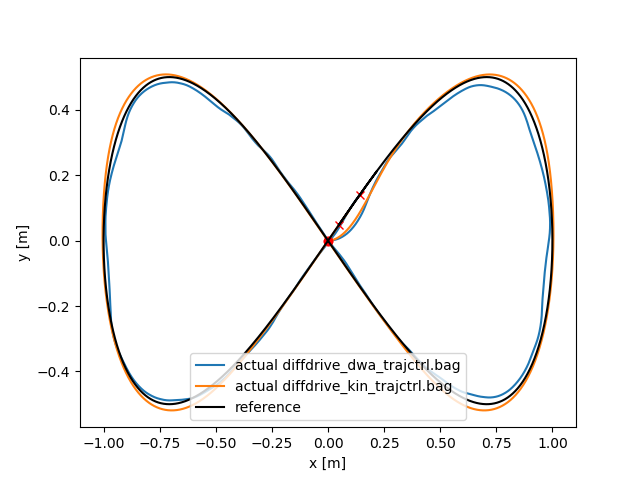
\includegraphics[scale=0.5]{comparison/Trajectory.png}
    }
    \quad
    \subfloat[Linear and angular velocities comparison.]{
        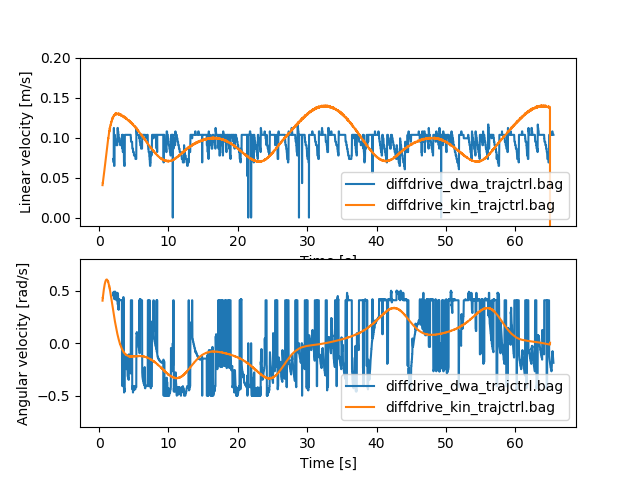
\includegraphics[scale=0.4]{comparison/Linear_and_Angular_Velocities.png}
    }
    \subfloat[Wheels velocities comparison.]{
        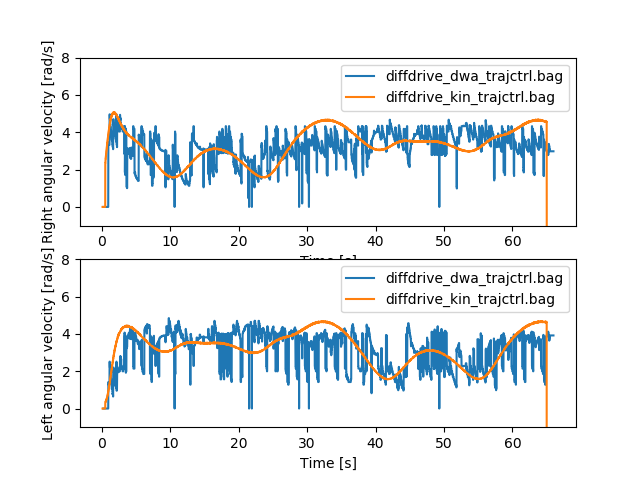
\includegraphics[scale=0.4]{comparison/Wheels_Velocities.png}
    }
    \quad
    \subfloat[Pose comparison.]{
        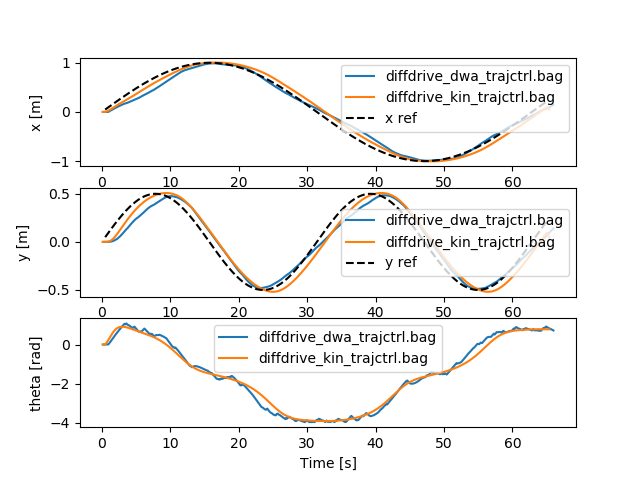
\includegraphics[scale=0.4]{comparison/Pose.png}
    }
    \subfloat[Position Error comparison.]{
        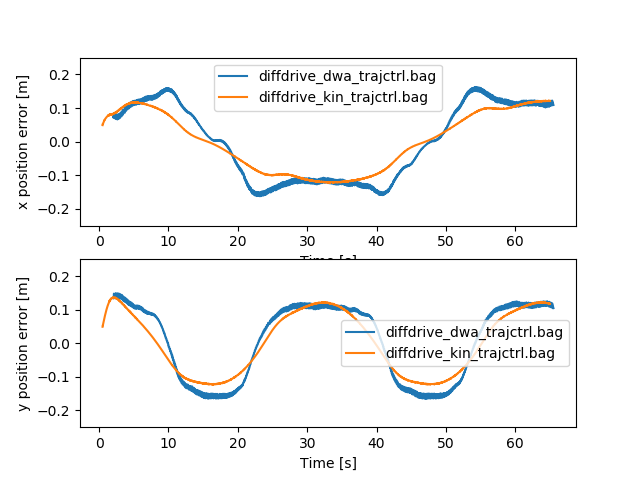
\includegraphics[scale=0.4]{comparison/Position_Error.png}
    }
    \caption[]{Comparison between the two approaches.}
\end{figure}




%--------------------------------------------------------------------------------------------------------------
%                                           ENCOUNTERED PROBLEMS
%--------------------------------------------------------------------------------------------------------------

\section{Encountered problems}


%------------------------------------------ DEPRECATED PARAMETERS ------------------------------------------

\subsection{Deprecated parameters}

During the tuning phase of DWA a trial and error approach has been carried out, finding that
a few parameters are named differently in the in the ROS library
\footnote{\href{https://docs.ros.org/en/melodic/api/dwa\_local\_planner/html/dwa\_\_planner\_\_ros\_8cpp\_source.html}{https://docs.ros.org/en/melodic/api/dwa\_local\_planner/html/dwa\_\_planner\_\_ros\_8cpp\_source.html}}
with respect to the ROS Wiki
\footnote{\href{https://wiki.ros.org/dwa\_local\_planner}{https://wiki.ros.org/dwa\_local\_planner}}.

Such renaming was not advertised by any error nor warning, so it was difficult to spot where the problem
was when changing parameters and seeing no effect in the robot behavior.

In fact, the warning would be raised only if DWA was instantiated inside the \texttt{nav\_core} architecture,
which is not the case when using DWA standalone.\\

The following pair of parameters is an example:
\begin{itemize}
 \item \texttt{min\_rot\_vel} renamed into \texttt{min\_vel\_theta};
 \item \texttt{max\_rot\_vel} renamed into \texttt{max\_vel\_theta}.\\
\end{itemize}

\begin{figure}[H]
    \centering
    \subfloat[ROS Wiki description.]{
        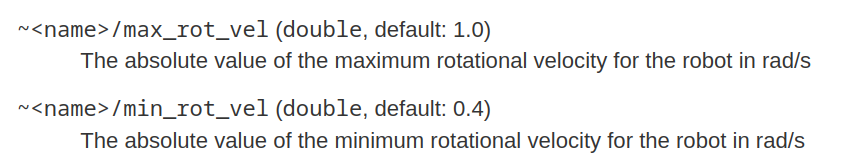
\includegraphics[scale=0.5]{other/deprecated_parameters_description.png}
    }
    \quad
    \subfloat[ROS library source code warning.]{
        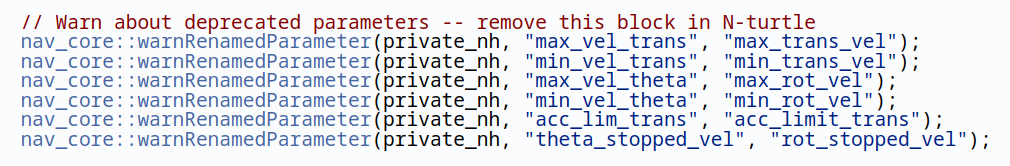
\includegraphics[scale=0.5]{other/deprecated_parameters_warning.png}
    }
    \caption[]{Deprecated parameters.}
\end{figure}


%------------------------------------------ DWA USED STANDALONE ------------------------------------------

\subsection{DWA used standalone}

Usually DWA is used inside a standard architecture which is the Navigation Stack in ROS.

However the goal of this project was to integrate DWA in the architecture with the simulator used for
the custom controller. Thereby DWA has been rearranged in a standalone mode.\\

To accomplish this, it has been necessary to provide to DWA all the information it normally expects on certain topics such as \texttt{/odom}, \texttt{/goal}, and \texttt{/map}.\\

Unfortunately there is no documentation for this kind of setup on the ROS Wiki, and the few lines of code that are present
refer to some deprecated libraries (i.e. \texttt{tf} is the one mentioned in the example, while \texttt{tf2} is the actual
supported one).

\begin{figure}[H]
    \centering
    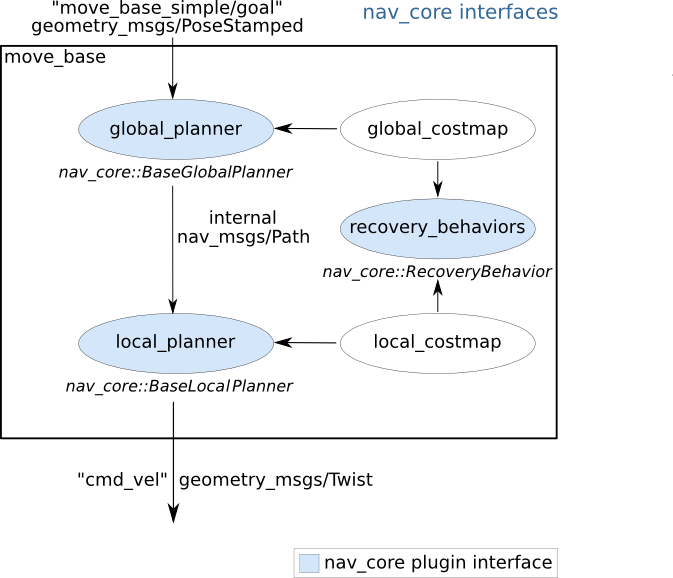
\includegraphics[scale=0.6]{other/nav_core.png}
    \caption{\texttt{nav\_core} package architecture.}
\end{figure}


%------------------------------------------ MULTIPLE GOALS ------------------------------------------

\subsection{Multiple goals}

In a standard scenario DWA needs only the one final goal and computes the trajectory on its own.

In this project the trajectory is predefined and must be forced changing continuously the goal, otherwise the robot
would go straight to the final point of the overall eight-shaped trajectory.




%--------------------------------------------------------------------------------------------------------------
%                                           USAGE OF THE CODE
%--------------------------------------------------------------------------------------------------------------

\section{Usage of the code}


%------------------------------------------ INSTALLATION ------------------------------------------

\subsection{Installation}

First of all, all the software written in this project has been tested on \textit{Ubuntu 18.04 LTS} and \textit{ROS Melodic}.\\

In order to install ROS and all the required packages, execute:

\begin{lstlisting}
sudo apt instal ros-melodic-desktop-full
sudo apt install ros-melodic-costmap-2d ros-melodic-base-local-planner ros-melodic-dwa-local-planner ros-melodic-map-server
\end{lstlisting}


%------------------------------------------ SETUP AND COMPILATION ------------------------------------------

\subsection{Setup and compilation}

Clone or download the repository into your home ($\sim$) folder.\\

If you use bash, add the following line to the end of your .bashrc:
\begin{lstlisting}
source ~/ROS_trajectory_tracking_controller/devel/setup.bash
\end{lstlisting}

If you use zsh, add instead this other line to the end of your .zshrc:
\begin{lstlisting}
source ~/ROS_trajectory_tracking_controller/devel/setup.zsh
\end{lstlisting}

Enter the project root directory and compile everything with:
\begin{lstlisting}
cd ROS_trajectory_tracking_controller
catkin_make
\end{lstlisting}


%------------------------------------------ SIMULATION AND RESULTS ------------------------------------------

\subsection{Simulation and results}

The following instructions let you perform and visualize a simulation.

\subsubsection{Custom controller}

This simulation shows the behavior of the custom controller when an 8-shaped trajectory is set.\\

\textit{[terminal 1]} Start the simulation:
\begin{lstlisting}
roslaunch diffdrive_kin_ctrl diffdrive_kin_trajctrl.launch
\end{lstlisting}


\textit{[terminal 2]} Enter the \texttt{script/} folder and record the simulation:
\begin{lstlisting}
cd ~/ROS_trajectory_tracking_controller/src/diffdrive_kin_ctrl/script
rosbag record -a -O diffdrive_kin_trajctrl.bag
\end{lstlisting}

Wait about 30 seconds so that the simulation can be performed.\\

\textit{[terminal 2]} Stop the recording with Ctrl-C.\\

\textit{[terminal 1]} Stop the simulation with Ctrl-C.\\

\textit{[terminal 2]} Visualize the results:
\begin{lstlisting}
python plot_results.py diffdrive_kin_trajctrl.bag
\end{lstlisting}

\subsubsection{DWA}

This simulation shows the behavior of DWA when an 8-shaped trajectory is set.\\

\textit{[terminal 1]} Start the simulation:
\begin{lstlisting}
roslaunch diffdrive_dwa_ctrl diffdrive_dwa_trajctrl.launch
\end{lstlisting}

\textit{[terminal 2]} Enter the script/ folder and record the simulation:
\begin{lstlisting}
cd ~/ROS_trajectory_tracking_controller/src/diffdrive_kin_ctrl/script
rosbag record -a -O diffdrive_dwa_trajctrl.bag
\end{lstlisting}

Wait about 30 seconds so that the simulation can be performed.\\

\textit{[terminal 2]} Stop the recording with Ctrl-C.\\

\textit{[terminal 1]} Stop the simulation with Ctrl-C.\\

\textit{[terminal 2]} Visualize the results:
\begin{lstlisting}
python plot_results.py diffdrive_dwa_trajctrl.bag
\end{lstlisting}

\subsubsection{Compare two simulations}

If you wish, you can also compare the results of two different simulations.

Given the two bag files named diffdrive\_dwa\_trajctrl.bag and diffdrive\_kin\_trajctrl.bag, visualize the comparison:
\begin{lstlisting}
python plot_comparison.py diffdrive_dwa_trajctrl.bag diffdrive_kin_trajctrl.bag
\end{lstlisting}




%--------------------------------------------------------------------------------------------------------------
%                                               CONCLUSIONS
%--------------------------------------------------------------------------------------------------------------

\section{Conclusions}











\end{document}
